\documentclass[final]{beamer}

\definecolor{redcaa}{RGB}{152,0,34}

\usepackage[orientation=landscape,size=a2,scale=1.5,debug]{beamerposter}  % e.g. custom size poster
\title{On the relationship between rabbit-skinners and poppy-chewers}
\author{Hardy Stones}
\institute{Human Language Technology and Pattern Recognition,RWTH Aachen University}
\date{April 2023}


% Set the font sizes for the headings and text
%\setbeamerfont{title}{size=\Huge}
%\setbeamerfont{author}{size=\huge}
\setbeamerfont{institute}{size=\large}
%\setbeamerfont{block title}{size=\Large}
%\setbeamerfont{block body}{size=\large}


% Remove the navigation symbols at the bottom of the poster
\setbeamertemplate{navigation symbols}{}

% Set the background color of the poster
\setbeamercolor{background canvas}{bg=white}
\setbeamercolor{block}{bg=white}
\setbeamercolor{structure}{fg=redcaa}

\setbeamercolor{block}{fg=black}
\setbeamercolor{block title}{fg=white,bg=redcaa}
\setbeamercolor{block body}{use=block title,bg=block title.fg}
\setbeamercolor{separation line}{bg=white,fg=redcaa}
\setbeamercolor{footline}{bg=redcaa,fg=white}
\setbeamercolor{footlinecolor}{fg=white,bg=redcaa}


\setbeamertemplate{footline}
{ 
    \begin{beamercolorbox}[wd=\paperwidth]{footlinecolor}
        \vskip5pt
        \begin{columns}
            \column{.05\paperwidth}
            \hspace{.2cm}
            
\includegraphics[height=2cm]{caa2023.pdf}
            \column{.75\paperwidth}
            CAA | April 2023 -- 
            \textcolor{white}{\textbf{On the relationship between rabbit-skinners and poppy-chewers}}
            Hardy Stone
            \column{.05\paperwidth}
            \hfil
        \end{columns}
        \vspace{.1cm}
    \end{beamercolorbox} 
}

% Begin the document
\begin{document}

% Create the title block
\begin{frame}[t]
    \vspace{-.5cm}
    \begin{beamercolorbox}[wd=\paperwidth]{block title}
    \vspace{.8cm}
        \begin{columns}

            \column{.15\textwidth}

            \column{.8\textwidth}
            {
                \raggedleft
                \usebeamerfont{title}\textcolor{white}{\textbf{On the relationship between rabbit-skinners and poppy-chewers}}\par
                \usebeamerfont{author}\textcolor{white}{Hardy Stone}\par
                \usebeamerfont{institute}\textcolor{black}{Institute of Normally Interesting \& Important Inquiries Carrying Evedicences}\par
            }

            \column{.05\textwidth}
            
\includegraphics[height=4cm]{uni2.png}
        \end{columns}
    \vspace{.8cm}

    \end{beamercolorbox}


    \vspace{2cm}


    \begin{columns}[t]

        \column{.22\textwidth}
% Create the first block
        \begin{block}{\textbf{Introduction}}
            Rabbit-Skinners and Poppy-Chewers were two distinct populations that inhabited the central and Western regions of Rabbithole during the prehistoric period from 7400BP to 6500BP. Despite their radically different subsistence strategies, both groups coexisted in the region for a significant period, and there has been much debate among archaeologists about the nature of their interactions.
        \end{block}
        \vspace{3cm}

% Create the second block
    \begin{block}{\textbf{Methods}}
            The authors developed a specific quantitative method called the ``Test of Balanced Equilibrium'' (TBE) to demonstrate the relationship between Rabbit-Skinners and Poppy-Chewers. The TBE equation is formulated as follows:

            \begin{equation}
                TBE = \sum_{i=1}^{n} \sum_{j=1}^{n} w_{ij} (N_i - N_j)
            \end{equation}

            In this equation, $N_i$ and $N_j$ represent the population sizes of two different settlements (or groups of settlements), and $w_{ij}$ is a weight that reflects the degree of interaction between these two settlements. This parameter will be fixed to 1 as the best tradeoff between complexity and accuracy.
        \end{block}

        \column{.45\textwidth}
% Create the third block
        \begin{block}{\textbf{Results}}
            The settlements were grouped into four different categories, and the TBE was calculated separately for each category. The results showed that Rabbit-Skinners and Poppy-Chewers had very intense and peaceful interactions despite their different subsistence strategies. The maps of Rabbit hole during the Old age (~7200 - 7000 BP) and after Farmer extension (~7000 - 6800 BP) are shown in Figures 1 and 2, respectively.

            \begin{figure}
                \label{fig:twomaps}
                \centering
                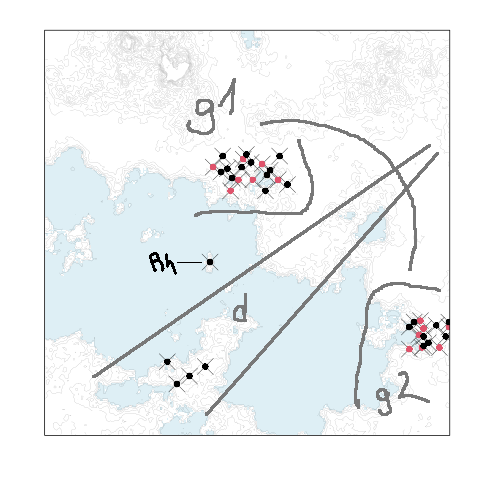
\includegraphics[width=.4\textwidth]{all_gpe}
                \makebox[.9\textwidth][c]{
                    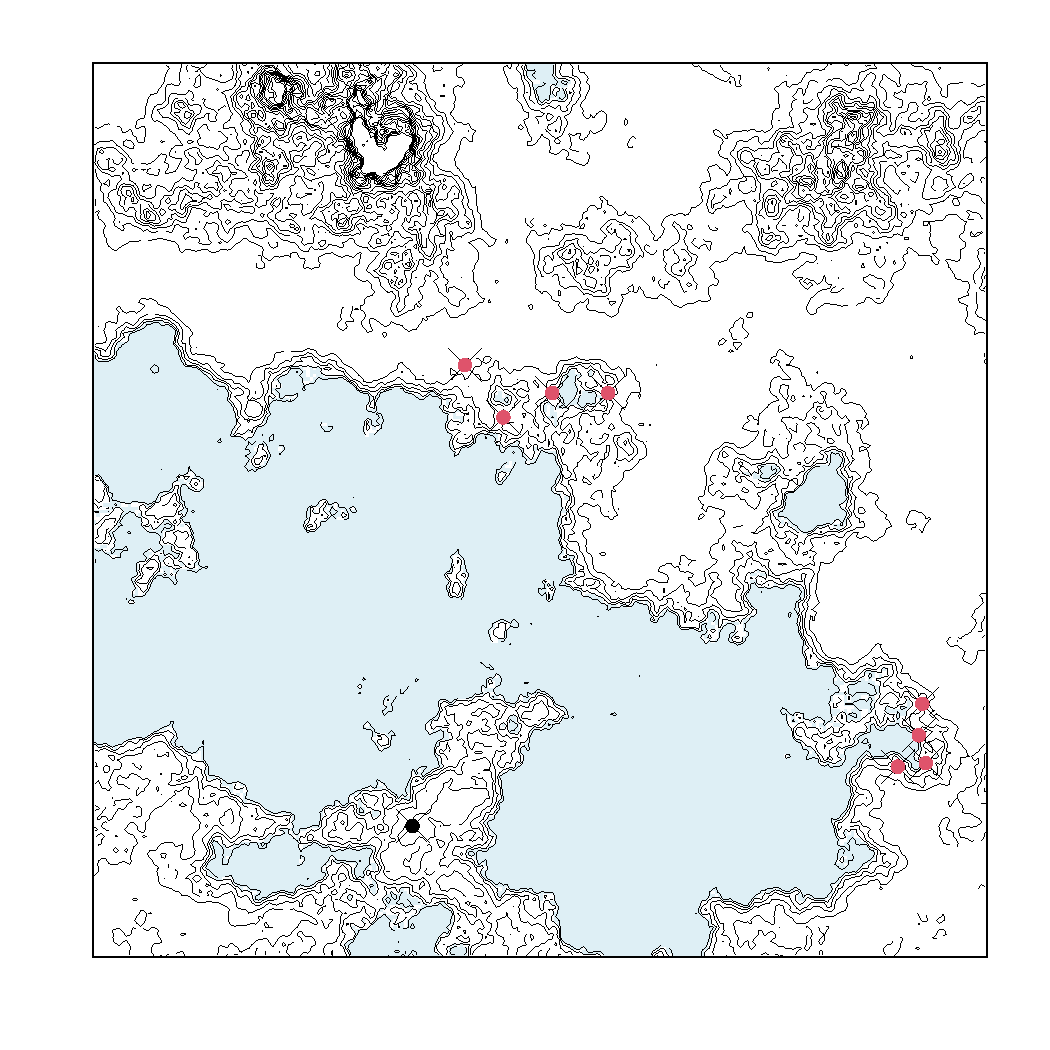
\includegraphics[width=.18\textwidth]{oldages}
                    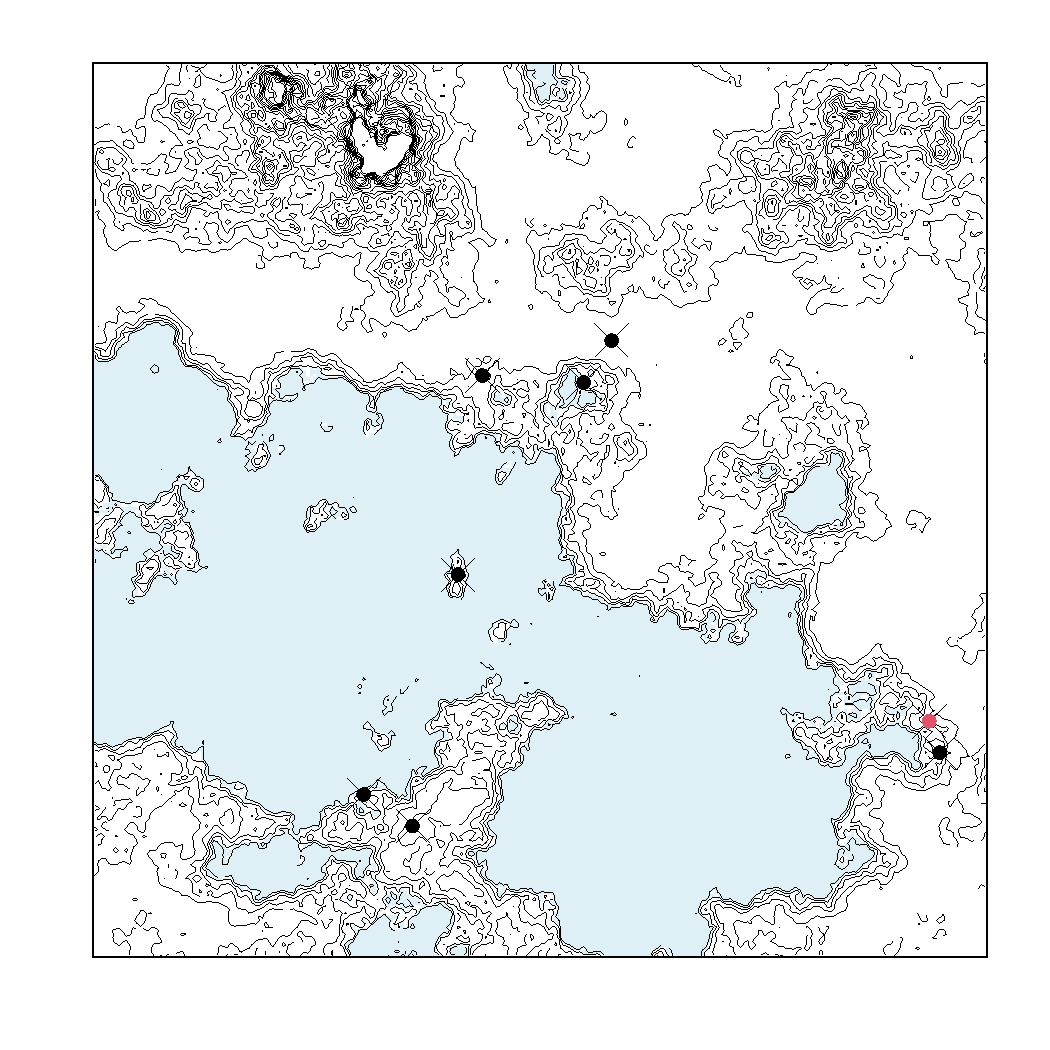
\includegraphics[width=.18\textwidth]{newages}
                }
                \caption{Map of rabbit hole during the Old age (~7200 - 7000 BP) on the left, after Farmer extension  (~7000 - 6800 BP) on the right }
            \end{figure}

        \end{block}

    \vfill
% Create the fourth block
    \begin{block}{\textbf{Conclusion}}
            The authors' TBE method provides a novel and powerful tool for studying the relationships between different populations in prehistoric times. The results of this study suggest that Rabbit-Skinners and Poppy-Chewers had a more symbiotic relationship characterized by trade and exchange rather than competition over resources. This study contributes to a better understanding of the history of Rabbithole and the nature of interactions between its inhabitants.
        \end{block}
        \column{.22\textwidth}

% Create the references block
        \begin{block}{\textbf{References}}
            Stone, H., \& Pants, F. (1966). Paleo-ecological reconstruction of Rabbithole environment during the between 8000BP to 6000BP. Journal of Ecological Research, 20(2), 45-56.
        \end{block}
        \vspace{8cm}
% Create the references block
    \begin{block}{\textbf{Additional note}}
        \small
    This project is part of the Archaoriddle project, funded by the British Academy - Leverhulme. If you want to help us understand what happened between Poppy-chewers and Rabbit-skinners flash the QR-code below. You will have a chance to receive a £650 grant to join us at the EAA in belfast! 
            \begin{figure}
                \includegraphics[width=.5\textwidth]{qrcode}
            \end{figure}
        \end{block}

    \end{columns}

\end{frame}
\end{document}


